\section*{\hypertarget{coc}{Caos en Cornelia}}
\addcontentsline{toc}{subsection}{Primera aventura}%
"¡Yo, Garland, acabaré con todos ustedes!" \\ 
\indent -- Garland \\\\ 
Caos en Cornelia es una aventura pregenerada que ofrece una introducción rápida y sencilla a Omega Fantasy. En esta aventura, el grupo tiene la tarea de encontrar a la princesa Sarah de Cornelia, que ha sido secuestrada. La trama se basa en el inicio del video juego Final Fantasy original del año 1987. Te recomendamos considerar todo este contenido como sugerencias y no como reglas, y que realices todos los cambios que consideres necesario. 

\subsubsection*{Primeros pasos}
Los jugadores pueden crear sus personajes siguiendo la \hyperlink{char}{Guía de creación de personajes}. El grupo comienza la aventura a bordo de un barco que viaja a Cornelia, por lo que cada personaje debería explicar por qué se sumaron en este viaje. Todos los personajes comienzan con el siguiente equipo en el nivel 1: Arma de Mythril o equivalente de nivel 1 que puedan utilizar, ropa, una poción y 100 Gil. El siguiente mapa muestra todos los lugares relacionados con la aventura.

\vfill

	\tcbox[left=0pt,top=0pt,right=0pt,bottom=0pt, boxsep=0pt, colframe=accent, sharp corners]{
	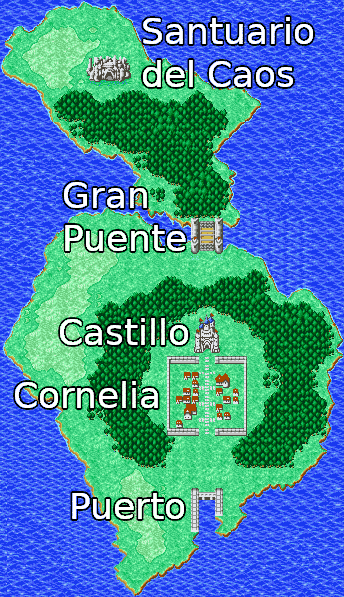
\includegraphics[width=0.98\columnwidth]{./art/maps/map.png} 
	}

\pagebreak

\subsection*{Viaje a Cornelia}
"¡Hasta la luna se cansa de dar vueltas esperando que muevan el trasero!"\\
\indent-- Cid 
\begin{center} 
	\tcbox[left=0pt,top=0pt,right=0pt,bottom=0pt, boxsep=0pt, colframe=accent, sharp corners]{
		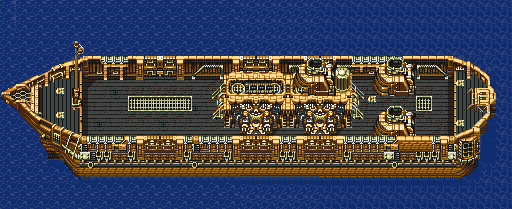
\includegraphics[width=0.98\columnwidth]{./art/maps/ship2.png} 
	}
\end{center}
La aventura comienza en un pequeño barco de transporte llamado "Pequeño Bronco", que está en camino de entregar carga a la ciudad de Cornelia. El capitán accedió a dejar que el grupo suba al barco por una pequeña tarifa. La tripulación del barco solo consta de 3 miembros: Biggs, Wedge y el capitán Cid. Los dos marineros llevan bandanas y pantalones cortos color celeste combinados con unas camisetas naranjas con rayas negras. Ambos son muy jóvenes e inexpertos, pero en general son amistosos con el grupo. No puede decirse lo mismo del viejo capitán, que se retiró a su camarote y prefiere que lo dejen solo. \subsubsection*{Día} "Aunque no lo parezca, soy todo un cobarde".\\
\indent-- Wedge \\\\
Si los aventureros no se conocen de antemano, deben presentarse primero, después de lo cual son libres de explorar el barco. También pueden hablar con los marineros que están felices de matar el tiempo durante el viaje. Biggs y Wedge les cuentan sobre recientes ataques piratas en altamar, que parecen haber aumentado recientemente. Además, también pueden darle al grupo novedades sobre Cornelia, ya que han oído que la princesa ha desaparecido. El grupo también puede preguntar sobre Cid, en cuyo caso los navegantes les cuentan su pasado como soldado. A medida que comienza a oscurecer, la tripulación se retira a sus cabinas. Los aventureros se preparan para terminar el día, cuando de repente se escuchan ruidos fuertes que rodean el barco. De inmediato se dan cuenta de que varios piratas han abordado al Pequeño Bronco. \subsubsection*{Batalla en el Pequeño Bronco} Coloca aproximadamente un pirata en el barco por cada miembro del grupo y distribúyelos alrededor de la plataforma como creas conveniente. La tripulación del barco está fuera de vista, luchando contra otros piratas que han entrado en el barco por debajo de la cubierta. Si las cosas se llegan a complicar para el grupo durante esta batalla, Biggs y Wedge pueden subir para ayudarlos. Sus detalles de combate se muestran a continuación. Son los mismos que los de los piratas. Después de derrotar a los enemigos, recuerda recompensar al grupo con el Gil que cada pirata derrotado dejó. Después de la batalla, la tripulación se reúne con el grupo y Cid les agradece su ayuda. Les explica que esta no es la primera vez que los atacan estos piratas, que son parte de la tripulación del capitán Bikke. Ahora, el grupo puede bajar a dormir para recuperar por completo sus PV y PM. Poco después de despertarse por la mañana, el barco llega a puerto de Cornelia. Una vez allí, la tripulación comienza a descargar la mercadería y se separa del grupo.
%
\vspace{0.5cm}
%
\monster{Pirate / Biggs / Wedge}{1}{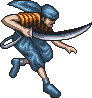
\includegraphics[width=0.16\textwidth]{./art/monsters/pirate.png}}
{
	HP: & \hfill 8 & MP: & \hfill 0\\
	STR: & \hfill 1 & DEF: & \hfill 0 \\
	MAG: & \hfill 0 & RES: & \hfill 0 \\
	AGI: & \hfill 3 & Size: & \hfill M\\
}
{
	\textbf{Scimitar}: 1d DMG \hfill \textbf{Drops:} 150 Gil 
}
%
\vspace{0.5cm}
%
\subsection*{Puerto de Cornelia}
El puerto de Cornelia es pequeño y tiene capacidad para un puñado de barcos de carga como el Pequeño Bronco. Los marineros del puerto están descargando cajas de los barcos, ya sea para almacenarlos en depósitos o llevarlos directamente a Cornelia. Luego de desembarcar, el grupo puede preguntar por el puerto cómo llegar a Cornelia. Los marineros les sugieren que tengan cuidado, ya que los guardias del castillo no están patrullando el camino. Cornelia no está lejos del puerto y el camino está rodeado principalmente de campos y prados.
%
\vfill
\tcbox[left=0pt,top=0pt,right=0pt,bottom=0pt, boxsep=0pt, colframe=accent, sharp corners]{
	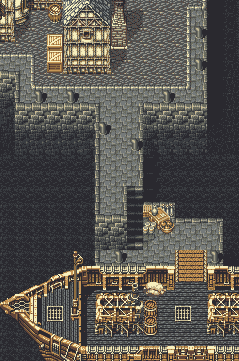
\includegraphics[width=0.98\columnwidth]{./art/maps/port.png} 
}
%
\subsubsection*{Dyce}
"Por cierto… ¿necesitan algo? ¡Echen un vistazo a mis productos! Es posible que se sorprendan con lo que encuentren..."\\
\indent-- Dyce \\\\
El grupo puede toparse en el puerto con un mercader errante llamado \textbf{Dyce}. Dyce es un hombre alto y fornido. Es calvo con barba y luce ropas oscuras. También tiene un \hyperlink{chocobo}{Chocobo} a su lado, que utiliza como medio de transporte. Le brinda información al grupo sobre los problemas de Cornelia, ya que ha oído rumores de que la princesa fue secuestrada. También vende Pociones a 125 Gil cada una, pero tiene más inventario que el grupo no puede permitirse en este momento. Dyce es un viajero, así que es probable que el grupo vuelva a encontrarse con él en el futuro. Sus precios suelen ser más altos en comparación con las tiendas habituales.

\subsubsection*{Batalla en el Puerto de Cornelia}
"¡Deben tener bolas de acero para desafiarme a mí!" -- Bikke \\\\
Al hablar con Dyce u otros marineros, el grupo se entera de que últimamente el puerto suele ser atacado por piratas. Normalmente el puerto está protegido por las guardias de Cornelia, pero desde la desaparición de la princesa, el rey ha replegado a todas las tropas al castillo. Los piratas siempre atacan por la noche y si grupo espera en los alrededores del puerto hasta que anochezca, en cualquier día, presenciaran un ataque de los piratas. Como el grupo lo sabe de antemano, pueden intentar adoptar medidas defensivas de antemano, como preparar una emboscada o trampas. El ataque comienza con un gran barco pirata que atraca en el puerto y varios piratas que despliegan para robar los depósitos y otros barcos. Los piratas son, una vez más, la tripulación del Capitán Bikke, pero esta vez también está presente el mismísimo Bikke. Durante la batalla, Bikke permanece detrás de las líneas ofensivas y se retira inmediatamente hacia su barco una vez que recibe cualquier daño. También hay algunos de sus hombres a su lado, de nuevo uno para cada miembro del grupo. Dado que es probable que Bikke escape de la batalla, el grupo puede volver a encontrarse con él en el futuro. Después de rechazar el ataque de los piratas, los marineros del puerto están muy agradecidos con el grupo y les ofrecen alojamiento y comida gratis por esa noche.
\vfill
\monster{Bikke}{2}{
\includegraphics[width=0.15\textwidth]{./art/monsters/pirate2.png}}
{
 PV: & \hfill 30 & PM: & \hfill 25\\
 FUE: & \hfill 1 & DEF: & \hfill 2 \\
 MAG: & \hfill 1 & RES: & \hfill 2 \\
 AGI: & \hfill 2 & Tamaño: & \hfill M\\
}
{
 \textbf{Cimitarra}: 1d de daño \mspell{Electro}{4}{0t}{Único}{3u}{Infliges 2d de daño \hyperlink{type}{Eléctrico} al objetivo}{\lightning} \mtech{Arenga}{5}{0t}{Único}{3u}{El objetivo recibe \hyperlink{status}{aumFUE} por 1 turno.}{\enstr} }

\clearpage
\subsection*{Cornelia}
A continuación se muestra el mapa de Cornelia, pero también hay granjas y edificios más pequeños fuera de las murallas de la ciudad que no se muestran. Todos los edificios están marcados con un número y puedes encontrar más detalles sobre ellos en los párrafos numerados. El grupo llega a Cornelia desde la puerta sur, donde dos guardias los detienen ya que no reconocen a los aventureros. Aconsejan al grupo alejarse del castillo y salir de la ciudad luego de terminar sus asuntos. La mayoría de los habitantes del pueblo está demasiado asustada como para dejar sus hogares desde que la princesa ha desaparecido.
\begin{center} 
	\tcbox[left=0pt,top=0pt,right=0pt,bottom=0pt, boxsep=0pt, colframe=accent, sharp corners]{
	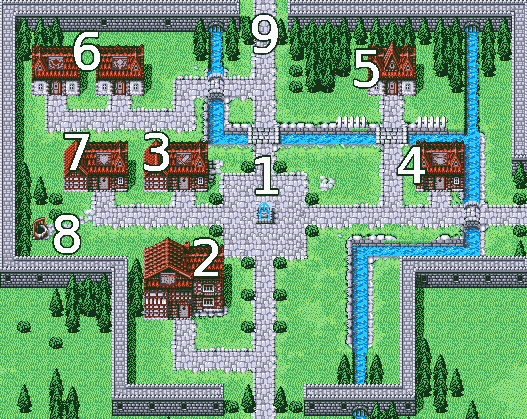
\includegraphics[width=0.98\columnwidth]{./art/maps/cornelia.png} 
	}
\end{center}
\subsubsection*{1 Fuente}
"¡Hola! ¡Soy una bailarina! ¿Qué dices? ¿Te gustaría un baile? Jijiji" -- Arylon \\ \\
El grupo observa una hermosa fuente que se destaca en medio de un pueblo por demás ordinario. En las cercanías se encuentra una joven alegre de cabello azul y vestido rojo practicando unos pasos de baile. Su nombre es Arylon. Cuando se le pregunta sobre la princesa o el castillo, revela los rumores que ha escuchado: han tomado de rehén a la princesa Sarah y piden un cuantioso rescate. En consecuencia, el castillo está inmerso en el caos y se le ha prohibido la entrada al público en general. También revela que ha habido múltiples intentos infructuosos de rescatar a Sarah. Observa las armas del grupo y les pregunta si estarían interesados en ayudar.

\subsubsection*{2. Posada}
"¡Pasen, por favor! Cobramos 50 Gil por noche. ¿Desean quedarse?" -- Elia \\\\
El grupo entra en una pequeña habitación con una alfombra roja en el suelo y un mostrador al final. Detrás del mostrador se encuentra una joven con pelo azul oscuro y un vestido largo verde. Su nombre es Elia. A la izquierda hay una amplia habitación donde los huéspedes duermen, con varias camas y pequeñas decoraciones en las paredes. A la derecha hay otra habitación, con sillas de madera y mesas donde los huéspedes pueden sentarse a comer y beber. Normalmente está sentado allí un viejo borracho llamado Argus y, a veces, unos pocos guardias. El grupo puede dormir en la posada por 50 Gil por noche por persona. También pueden pedir información a Elia, ya que escucha muchos comentarios de los visitantes. Ella le informa al grupo sobre varias personas del pueblo que pueden necesitar ayuda, como el herrero y los magos. El grupo también puede hablar con Argus, que balbuceará historias sobre un gran soldado llamado Garland que él conocía de cuándo era un guardia.

\subsubsection*{3. Herrero}
El grupo entra en una gran tienda con una forja, donde se exhiben muchas armas y armaduras. Detrás del mostrador hay un hombre viejo de pelo castaño y barba larga. Su nombre es Todo. Les dice al grupo que la tienda está cerrada: no puede trabajar debido a que no recibe la mercadería necesaria que fue enviada al puerto. Para ayudarlo, el grupo tiene que hablar con Dyce en el puerto de Cornelia, que está controlando a los envíos. El envío de Todo consiste en una caja de madera grande en un pequeño carro, que disminuye un poco el paso del grupo. En el camino de regreso, un extraño monstruo llamado PuPu intenta robar los envíos. PuPu está sentado en los árboles y utiliza su habilidad "Abducir" para hacer desaparecer lentamente la caja. Si los jugadores lo buscan en los árboles mientras él hace esto, es fácil de detectar, ya que la parte superior de su cabeza resplandece. Después de eso, es difícil de detectar: un jugador tiene que tener éxito en una tirada que puede variar entre una DC 6 y 8. Puede que el grupo no encuentre PuPu, pero estará cerca si regresan al mismo lugar en otro momento. Si se detecta, PuPu no lucha, sino que pide Pociones (consulte "¡Pociones, por favor!") y devuelve los artículos robados si el grupo las concede. También puedes recompensar al grupo por resolver la disputa pacíficamente: PuPu puede, por ejemplo, devolver artículos adicionales o Gil. El grupo también puede atacarlo, en cuyo caso el envío vuelve a aparecer después de derrotar a PuPu. Al entregar el envío, Todo recompensa al grupo con 500 Gil. El herrero puede empezar a trabajar de nuevo, pero estará ocupado completando pedidos pendientes durante algún tiempo. Cuando el grupo regrese en unos días, Todo puede mejorar sus armas o armaduras y puede vender cualquier arma o armadura de nivel 1 a elección.
\vfill
\friendly{PuPu}{???}{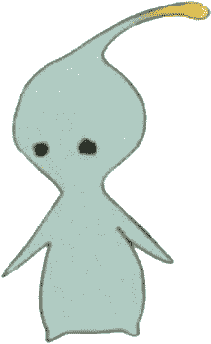
\includegraphics[width=0.13\textwidth]{./art/monsters/pupu.png}}
{
	HP: & \hfill 10 & MP: & \hfill 10\\
	STR: & \hfill 0 & DEF: & \hfill 0 \\
	MAG: & \hfill 0 & RES: & \hfill 0 \\
	AGI: & \hfill 2 & Size: & \hfill S\\
}
{
	\textbf{Drops}: All abducted objects 
	
	\mtech{Abduct}{0}{1r}{Single}{5u}{
		An object that you can see within range disappears to an unknown location.  
	}{}	
	\mpassive{Potion Please!}{
		Ask your enemies to give you a \hyperlink{item}{Potion}, if they comply make a DC 8 check.
		If you succeed you disappear to an unknown location (\hyperlink{status}{KO}), otherwise you keep asking for more \hyperlink{item}{Potions}.
	}
}

\subsubsection*{4. Tienda}
Esta tienda de artículos generales está compuesta por un gran mostrador en el centro y varios objetos y productos a su alrededor. Detrás del mostrador hay un hombre joven de pelo oscuro con una bandana verde. Su nombre es Guston. No está particularmente preocupado por la princesa, pero está molesto porque los problemas en Cornelia han afectado a sus ventas. En consecuencia, es muy agradable con posibles clientes y vende los elementos que se indican a continuación. Además, puede tener cualquier otro objeto que quieras en su inventario.
%
\vspace{0.1cm}
%
\consumables{Objetos}{item2.png}{
 \hline Poción & 100 Gil & Recupera 2d de PV. \\ 
 \hline Ala de \newline Fénix & 250 Gil & Recupera el estado \hyperlink{status}{KO} y recupera 1 PV.\\ 
 \hline Carpa & 500 Gil & Permite al grupo descansar en las afueras. \\
 \hline Linterna & 100 Gil & Una linterna normal. \\ 
} 

\subsubsection*{5. Capilla}
"No pierdan el valor, valientes guerreros".
\indent -- Gregory\\\\
La capilla es pequeña y acogedora con pocos bancos de madera, pero también está completamente vacía, salvo por una persona, el padre Gregory. Gregory es un viejo de barba larga y blanca que lleva una túnica roja con capucha. Habla muy despacio y lento. Se lamenta que nadie ha visitado la capilla desde la desaparición de Sarah. Aparentemente, la mayoría de los habitantes del pueblo creen que el incidente es un castigo divino, por lo que no se acercan a la capilla. El padre le pide al grupo que restablezca la fe en el pueblo de Cornelia. El grupo puede convencer a las personas, por ejemplo, dando detalles sobre la desaparición de Sarah (fue secuestrada) que muchos no saben, ya que desde el castillo no dieron ningún tipo de información. Si el grupo consigue convencer al menos a 3 personas de Cornelia que asistan a la capilla, Gregory estará satisfecho y los recompensará con 500 Gil. Además, ofrece sus servicios de manera gratuita al grupo: puede curar el estado \hyperlink{status}{KO} realizando un ritual de 1 hora.

\subsubsection*{6. Los magos}
Estos dos edificios son casi idénticos: ambos tienen una sola habitación grande con una cama y estantes con montones de productos y libros de magia y alquimia. Están habitadas por dos excéntricos y testarudos gemelos: Gilles y Noah. Gilles es un mago negro que viste una bata azul y un sombrero en punta, mientras que Noah es un mago blanco que lleva una bata blanca con capucha con detalles rojos. El resto de los habitantes del pueblo evita los hermanos, excepto cuando necesitan de sus servicios. Esto los irritaba, así que los magos decidieron desarrollar un frasco especial que les permite almacenar su magia para que otros puedan usarla sin su presencia. Desafortunadamente, algo salió mal durante su desarrollo, lo que provocó que el objeto explotara violentamente. El grupo puede ver los restos en el patio trasero. Siendo ambos tan orgullosos, se culpan entre ellos por el accidente y se han dejado de hablar desde entonces. El grupo puede resolver la disputa convenciéndolos de que ambos son culpables. Por ejemplo, pueden lograr esto de la siguiente manera: Primero, tienen que reparar el frasco roto a través de medios mecánicos o mágicos, que es fácil. Después, tienen que estudiar el frasco y la receta para crearlo, que pueden conseguir de los magos. Al hacerlo, un personaje que pueda utilizar magia entiende el problema. Un personaje que no pueda usar magia tiene que pasar una tirada con DC 8. El frasco se rompió porque después de crearlo, cada mago lanzó 2 hechizos, lo que provocó que el frasco se sobrecargara (solo puede contener un total de 3 hechizos como máximo). Esto se puede demostrar lanzando solo 3 hechizos en el frasco, que en efecto funciona bien. Si el grupo consigue convencer a los magos, aceptan su error y se disculpan entre sí. Le regalan el frasco al grupo como una muestra de gratitud y el grupo puede visitarlos en el futuro para comprar los accesorios que se muestran a continuación, a los que puedes añadir cualquier otro a elección.
%
\vspace{0.3cm}
%
\accessory{Accesorios}{acc.png}{
 \hline Frasco \newline Mágico & 1000 Gil & Puede almacenar hasta 3 hechizos que se le lancen. Quien lo lleve puede usar una acción para liberar un hechizo almacenado en el objetivo elegido. \\ 
 \hline Brazletes \newline Rúnicos & 500 Gil & RES +1 \\
 \hline Escudo \newline de Mithril & 500 Gil & DEF +1 \\ 
} 

\subsubsection*{7. Edificio abandonado}
Este edificio está vacío a propósito, en caso de que lo necesites. Por ejemplo, puede estar relacionado con una de los historias de algún personaje o puede alojar personajes o contenido que desees añadir a la aventura. Si no lo utilizas, la casa está vacía y los jugadores pueden preguntar por la ciudad para descubrir que solía ser una tienda que ha sido abandonada ya que no era rentable. Si el grupo logra traer de regreso a la princesa sana y salva, el rey puede también obsequiarles esa casa como recompensa. Será muy útil si el grupo regresa a Cornelia en un futuro o pueden vendérsela a alguien más. 

\subsubsection*{8. Pozo}
Es un pozo. Parecería que se puede descender por él, pero no se puede. En serio. 

\subsubsection*{9. Entrada al castillo}
Esta entrada conduce directamente al castillo de Cornelia y está protegida día y noche por al menos 4 guardias que no permiten que nadie pase. Sin embargo, les permiten la entrada a los aventureros si estos les explican que quieren ayudar a encontrar a la princesa. A continuación, los guardias le piden al grupo que se presente ante el canciller en la planta superior para obtener más información.

\pagebreak
\subsection*{Cornelia Castle}
A map of the ground floor is shown below, where relevant locations are numbered according to their paragraphs.
The stairs in the center lead to the throne room, while the entrance in the back leads to the palace garden, which is currently closed off.
The palace is filled with armed guards at all times.
\begin{center} 
	\tcbox[left=0pt,top=0pt,right=0pt,bottom=0pt, boxsep=0pt, colframe=accent, sharp corners]{
		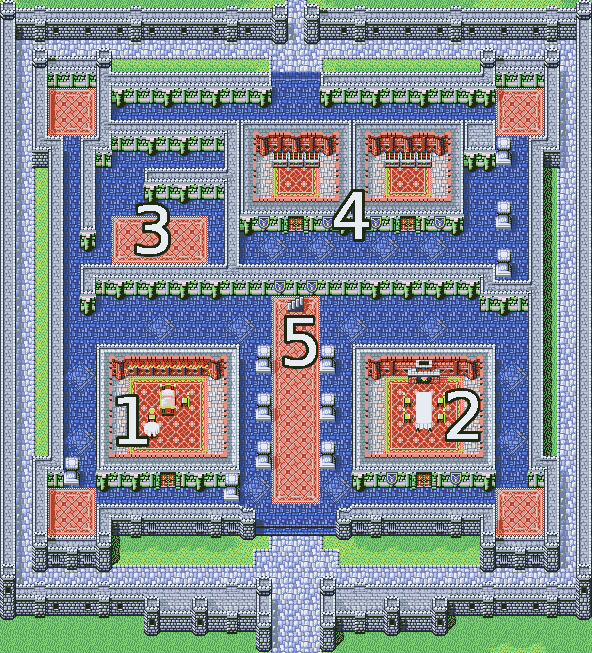
\includegraphics[width=0.98\columnwidth]{./art/maps/castle.png} 
	}
\end{center}
\subsubsection*{1. Queen's Room}
"Please... please bring my daughter... my Sarah... back to me safely."
\indent -- Queen Jayne \\\\
Queen Jayne is a middle-aged women with turquoise hair and blue eyes, wearing a well-made long red dress and a golden tiara.
She has been depressed since her daughter's kidnapping and only talks to the party after they have won the king's trust.
Once she talks, she tells the party about the night of the kidnapping, which she has witnessed personally.
On that night, she woke up and encountered Garland who was escaping with the unconscious princess in his arms.
Garland told her to hand over control Cornelia if she wants to see her daughter alive again.
Then he disappeared with Sarah through the back entrance of the palace.
The Queen is traumatized by this event and she blames herself for not preventing the kidnapping.

\subsubsection*{2. Sisters's Room}
"My s-s-sister... W-where's my s-sister?"
\indent -- Alison\\\\
This room is inhabited by Sarah's sister Alison who is an emotional teenager, that resembles her mother.
The guards at her door tell the party that she has locked herself in and won't open the door.
If the party can convince her, e.g. by assuring that they will save Sarah, she opens the door to talk.
Alison knows her sister well, as she looks up to her very much.
She tells the party about Sarah's passion for music and that her precious lute has disappeared with her.
If the party manages to calm Alison down, they have a better chance at convincing the king, who is worried about her. 

\subsubsection*{3. Captain}
"Garland was once the greatest knight in the kingdom. But power corrupted him, and he turned away from his own true nature."
\indent -- Ian \\\\
The captain of the guard is a young man with long blond hair named Ian, he is wearing a decorated heavy armor and a longsword on his back.
He is reluctant to talk the adventurers and they immediately notice that he is missing his left arm. 
If the party has convinced the king, the captain is willing to talk to them about the mission to rescue Sarah, which he led.
Right after Sarah disappeared, him his men followed Garland and confronted him at the Big Bridge, north of Cornelia.
However, Garland bested all of them in ensuing battle and the captain was the only one to survive, albeit without his arm.
He is ashamed of his failure and seems deeply disturbed and scared of Garland's power.

\subsubsection*{4. Treasure Room}
The treasury consists of two rooms, the one to the left contains the palace's gold while the right one contains expensive items and equipment.
Both doors are guarded by two well armed men in heavy armor.
If the party has obtained a letter from the king, they are given the following items by guards: 
A large Tent that fits the entire party as well as a Potion and 200 Gil per party member.

\subsubsection*{5. Throne Room}
The door is guarded by two royal guards with glaives and heavy decorated armor.
Inside the throne room, the king sits on his throne and beside him stands the chancellor.
The king is a middle-aged man with light blue eyes and brown hair with a long brown beard, he is wearing a golden crown and long red robes.
The chancellor is slightly younger with dark hair, also wearing noble clothing.
The king is happy to see the adventurers, as he is desperate to find his daughter, but the chancellor is very skeptical.
In the following conversation, the party can try to convince the king that they can rescue Sarah, but the chancellor convinces him that they have to prove their trustworthiness first.
The king then laments that he has been neglecting his people while trying to rescue his daughter.
He asks the party to help the people of Cornelia to prove that they are capable of saving Sarah, in return he promises to provide them with supplies for the journey.
If the party asks for further details on the kidnapping, they do not reveal anything until the party has won their trust.

\subsubsection*{Convincing the King}
"Garland is no longer the man I once knew... I beg of you. Please return my daughter to me quickly!"

\indent -- King of Cornelia \\\\
To convince the king, the party has to fulfil a number of tasks that help the people of Cornelia, which ones and how many exactly depends on you as the GM.
Below is a list of tasks that may convince the king if taken care of:
\begin{itemize}[leftmargin=*]
	\item Help the smith to receive his shipments.
	\item Resolve the dispute between the two mages.
	\item Defend the port against an ambush by pirates.
	\item Help the chapel regain its members.
\end{itemize}
After the party wins the king's trust, he reveals further details on the kidnapping:
Sarah was kidnapped by a former knight of Cornelia named Garland, the most powerful swordsman in the kingdom.
Garland used to be close to the king, but power has corrupted him and he demanded to become his successor. 
When the king denied him, Garland abducted his daughter Sarah as ransom for control over Cornelia.
Many other knights have tried to save her since and even though none succeeded, they found out that Garland keeps Sarah in the Chaos Shrine, north of Cornelia past the Big Bridge.
The king keeps his promise and writes a letter to confirm that they were officially given the task of rescuing the princess.
This letter allows the party to retrieve supplies from the treasury and other members of the palace are more willing to talk to them.
After successfully convincing the king, the party is rewarded with a \textbf{Level Up}!
\vspace{1.2cm}
\subsection*{Gran Puente}
"¡Veamos cómo se las arreglan contra el poderoso yo! ¡Y por "yo" me refiero a Gilgamesh! ¡Y por "se las arreglan", quiero decir SE MUEREN!" \\
\indent -- Gilgamesh \\\\
\noindent
Al salir de Cornelia y dirigirse hacia el norte, el grupo se encuentra en los bosques y prados que rodean la ciudad. Después de varias horas de viaje en la tranquilidad de la naturaleza llegan al Gran Puente, que es enorme pero también viejo y quebradizo. Cuando llegan al final del puente, se encuentran con Gilgamesh, que parece haber estado esperándolos. Gilgamesh no es ni bueno ni malo necesariamente. Viaja por el mundo para encontrar armas poderosas para su colección. Garland ha convencido a Gilgamesh para que trabaje para él y le ordena que proteja el puente de cualquier persona que intente cruzar. A cambio, Garland le regaló la legendaria espada Excálibur (o al menos eso es lo que Gilgamesh cree). Al encontrarse con el grupo, Gilgamesh los reconocerá como oponentes potencialmente dignos y desenvainará sus armas.
\pagebreak

\tcbox[left=0pt,top=0pt,right=0pt,bottom=0pt, boxsep=0pt, colframe=accent, sharp corners]{
	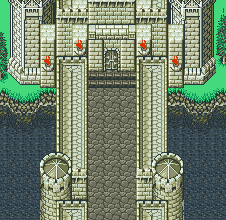
\includegraphics[width=0.96\columnwidth]{./art/maps/bridge.png} 
}

\subsubsection*{Batalla en el Gran Puente}
La batalla contra Gilgamesh tiene lugar al final del puente, como se muestra en el mapa anterior. A continuación se muestran sus características de combate, pero dependiendo del grupo, es posible que tengas que modificar algunos de sus atributos. Cuando los PV de Gilgamesh llegan a 0, no pierde el conocimiento sino que finalmente desenvaina la espada Excálibur para un último ataque. Intenta atacar al miembro más cercano con ella, pero la espada no provoca daño y se destruye inmediatamente. Gilgamesh se da cuenta de que Garland lo ha engañado. Sin otra opción a la vista, decide huír. Como sigue vivo, el grupo puede volver a encontrarse con Gilgamesh en el futuro. Después de derrotar a Gilgamesh, el grupo puede cruzar el puente para llegar al bosque oscuro antes del Santuario del Caos. El bosque está inusualmente silencioso y la mayoría de sus árboles y plantas parecen haber muerto. Es muy probable que los aventureros no lleguen al Santuario antes de la puesta de sol, por lo que probablemente tendrán que pasar la noche en el bosque.

\vspace{0.5cm}

\monster{Gilgamesh}{2}{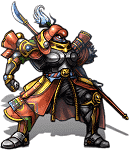
\includegraphics[width=0.17\textwidth]{./art/monsters/gilgamesh.png}}
{
 PV: & \hfill 45 & PM: & \hfill 40\\
 FUE: & \hfill 2 & DEF: & \hfill 1 \\
 MAG: & \hfill 0 & RES: & \hfill 0 \\
 AGI: & \hfill 4 & Tamaño: & \hfill M\\
}
{
 \textbf{Arma de Asta}: 1d de daño \hfill \textbf{Botín}: 500 Gil 
 
 \mtech{Garra Letal}{6}{0t}{Único}{Arma}{
 Realiza dos \hyperlink{action}{Ataques} contra el objetivo. Si al menos uno de ellos lo golpea, queda \hyperlink{status}{Inmóvil} por 1 turno. }{\immobile} \mtech{Danza de Espadas}{8}{1t}{3u}{Tú}{Realiza un \hyperlink{action}{Ataque} contra todos los enemigos dentro del área de efecto.}{}
 \mreaction{Poder Crítico}{Cuando tus PV sean menos de 20, recibes \hyperlink{status}{aumFUE} hasta el final de la batalla.} 
}

\pagebreak
\subsection*{Santuario del Caos}
Cuando el grupo llega a los prados que limitan con el Bosque Oscuro, alcanzan a ver el intimidante Santuario del Caos a la distancia. A medida que se acercan, notan que la naturaleza se ha adueñado del santuario, pues sus paredes están dañadas y cubiertas de vegetación. Los cimientos del edificio han comenzado a sumergirse en el suelo. Una serenidad anormal rodea el santuario. No hay rastro de vida a la vista y la única entrada es un conjunto de escaleras quebradizas que bajan hacia la oscuridad. Después de bajar las escaleras, el grupo llega al sur del mapa que se muestra a continuación y apenas puede ver en la oscuridad. El sector norte está bloqueado por escombros provenientes de las columnas y del techo. Tras una inspección más cercana, el grupo se da cuenta de que este bloqueo no fue accidental, si no que alguien lo ha hecho a propósito.
\vspace{0.1cm}
\tcbox[left=1pt,top=1pt,right=1pt,bottom=1pt, boxsep=-1pt, colframe=accent, sharp corners]{
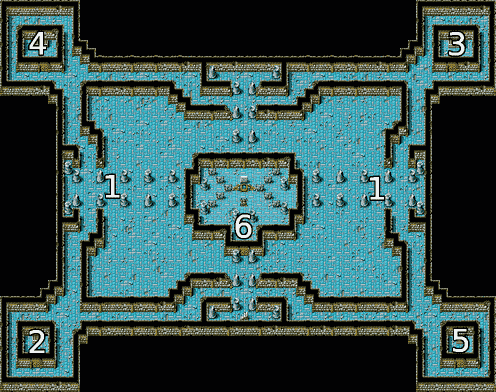
\includegraphics[width=0.98\columnwidth]{./art/maps/shrine.png}}

\subsubsection*{1 Trampas}
Ambas ubicaciones marcadas contienen una trampa mágica en el suelo que ha sido colocada por Garland para alertarlo e impedir que ingresen intrusos. Un personaje que esté activamente buscando trampas o que tome recaudos similares, notará la trampa mediante una tirada de DC 7. La trampa explota al pisarla e inflige 2d de daño de \hyperlink{type}{fuego }daños a todas las personas en un radio de 1u de su centro. \subsubsection*{2. Mímico}
Dentro de esta habitación hay un enorme cofre que al tocarlo se revela como un despiadado Mímico. Un personaje puede notar de antemano que hay algo extraño en el cofre pasando una tirada con DC 9. Si no tiene éxito, el Mímico obtiene automáticamente el mejor resultado posible en su tirada de iniciativa en la batalla.
\vfill
\monster{Mimic}{2}{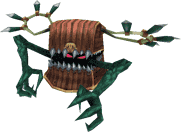
\includegraphics[width=0.25\textwidth]{./art/monsters/mimic.png}}
{
	HP: & \hfill 20 & MP: & \hfill 0\\
	STR: & \hfill 2 & DEF: & \hfill 0 \\
	MAG: & \hfill 0 & RES: & \hfill 0 \\
	AGI: & \hfill 2 & Size: & \hfill M\\
}
{
	\textbf{Bite}: 1d DMG \hfill \textbf{Drops:} 200 Gil	
}

\subsubsection*{3. Fuente de la sanación}
La pesada puerta de esta habitación está bloqueada y se puede destruir o forzar su cerradura pasando una tirada con DC de entre 6 y 9, dependiendo de la pericia del personaje. En esta habitación, el grupo encuentra un enorme cáliz que se encuentra en un pedestal de piedra lleno de lo que parece ser agua. Luego de una inspección más cercana, un personaje puede deducir que el líquido es de naturaleza mágica y que si alguien lo bebe, recupera por completo sus PV y PM inmediatamente. Sin embargo, el cáliz en sí no tiene propiedades mágicas y contiene solo 5 dosis del agua curativa. \subsubsection*{4. Cofres}
Esta sala contiene 2 cofres. Uno se puede abrir fácilmente y contiene 3 \hyperlink{item}{Pociones} y un \hyperlink{item}{Ala de Fénix}. El otro contiene el \textbf{Laúd de Sarah }y solo puede abrirse mediante una tirada con una DC que varía entre 7 y 10 según la pericia del personaje. También puede abrirse con una llave que Garland lleva consigo, pero el cofre es demasiado duro como para romper a la fuerza. \subsubsection*{5. Puerta secreta}
Esta sala está vacía, salvo por una gran lápida de piedra incrustada en la pared izquierda con varios símbolos diferentes. Después de una inspección más cercana, el grupo puede deducir que los símbolos describen una corta partitura de música. En la pared junto a ella hay una puerta secreta que se revela tocando la partitura con el Laúd de Sarah, y solo ella debería poder interpretar la melodía correctamente. La puerta secreta conduce a una pequeña sala con un pedestal de piedra que tiene el siguiente objeto: 
\vspace{0.3cm}
\accessory{Accesorios}{acc.png}{
 \hline Anillo \newline de Ángel & 2000 Gil & Si tienes este anillo equipado cuando caigas en estado \hyperlink{status}{KO}, puedes activar su efecto inmediatamente y volver a estar de pie con 1 PV. El anillo se destruye después de usar este efecto. \\
} 
%\pagebreak
\subsubsection*{6. Garland}
"Ahhh... los perritos falderos del rey. ¿Tienen idea de con quién se están metiendo?"
\indent -- Garland \\\\ 
En el centro del templo, el grupo finalmente se enfrenta a Garland. Sarah también está en esta habitación, encerrada en una jaula que se encuentra en una esquina. Garland es un hombre alto y fornido. Viste una armadura pesada y una capa morada y está armado con una espada. Es muy arrogante y cree que merece gobernar Cornelia porque es el guerrero más fuerte del reino. Desde que llegó, Garland ha estudiado los secretos oscuros del Santuario del Caos para aumentar su propio poder. Considera al grupo tan solo como una piedra más en el camino de sus grandes planes. \subsubsection*{Batalla final}
"¿Realmente creen que pueden enfrentarse a MÍ? De acuerdo…" \\
\indent -- Garland \\\\ 
Garland desenvaina su arma para comenzar la batalla y también invoca varios murciélagos para que lo asistan, uno por cada miembro del grupo. Durante la batalla, su posicionamiento se centra en arrinconar a los miembros del grupo individualmente mientras evita que lo superen en número. Prefiere que primero sus esbirros utilicen sus habilidades de larga distancia para luego intentar acabar con los enemigos que han sido debilitados. En la historia original, Garland utiliza un artefacto mágico para escapar después de ser derrotado y se convierte en el principal antagonista del juego. Si quieres continuar la aventura de forma diferente, también puede morir a mano de los aventureros o puedes dejar que los jugadores decidan su destino. Después de ser liberada de su prisión, Sarah sigue lógicamente muy asustada y traumada. Le agradece al grupo por rescatarla y les pide que encuentren su precioso laúd que Garland robó. El grupo puede rechazar su solicitud para regresar rápidamente a Cornelia. Sarah comprenderá pero no estará contenta.

\vfill
\monster{Murciélago}{1}{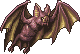
\includegraphics[width=0.18\textwidth]{./art/monsters/bat.png}}
{
 PV: & \hfill 6 & PM: & \hfill 0\\
 FUE: & \hfill 0 & DEF: & \hfill 0 \\
 MAG: & \hfill 0 & RES: & \hfill 2 \\
 AGI: & \hfill 4 & Tamaño: & \hfill P\\
}
{
 \textbf{Dientes}: 1d de daño \hfill \textbf{Botín:} 100 Gil 
 
 \mpassive{Absorber}{Por cada \hyperlink{action}{Ataque} exitoso, recuperas 1d de PV.} 
}
\vfill
\monster{Garland}{3}{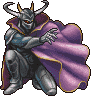
\includegraphics[width=0.18\textwidth]{./art/monsters/garland.png}}
{
 PV: & \hfill 40 & PM: & \hfill 30\\
 FUE: & \hfill 3 & DEF: & \hfill 1 \\
 MAG: & \hfill 1 & RES: & \hfill 1 \\
 AGI: & \hfill 2 & Tamaño: & \hfill M\\
}
{
 \textbf{Espada Larga}: 1d de daño \hfill \textbf{Botín}: 1000 Gil, Llave 
 
 \mspell{Absorber}{8}{1t}{Único}{3u}{ Reduces 1d de los PV del objetivo y recuperas tus PV por el mismo valor.}{} \mspell{Silencio}{6}{1t}{Único}{3u}{El objetivo hace una tirada con DC 8. Si falla, sufre \hyperlink{status}{Silencio} por 3 turnos.}{\silence}
 \mreaction{Parada}{Cuando falles al intentar esquivar un \hyperlink{action}{Ataque}, Puedes hacer una tirada con DC~8. Si tienes éxito, el daño que recibes se reduce a la mitad.}
}
\vspace{2.2cm}
\pagebreak

\subsection*{Epílogo}
"¿Han... han venido a rescatarme? No sé cómo puedo darles las gracias..." \\ 
\indent -- Sarah \\\\ 
Después de rescatar a Sarah, el grupo debe regresarla sana y salva a Cornelia y, por lo tanto, tienen que volver a atravesar el largo camino que recorrieron para llegar al Santuario. El viaje debería ser en general tranquilo, pero si quieres puedes añadir algunas sorpresas. Sarah es una princesa joven con pelo turquesa como su madre y luce un vestido dorado y un colgante dorado adornado con joyas rojas. Es educada pero también muy tranquila y ausente: el secuestro ha dejado cicatrices físicas y mentales en ella. Sarah no es capaz de cuidar de sí misma, así que necesita ayuda y orientación de los aventureros durante el viaje. Durante el viaje, a menudo pregunta por Cornelia y su familia, mientras se culpa por todo lo que ha sucedido. 

\subsubsection*{Llegada}
"Gracias por traer a mi hija de nuevo a mi lado". \\ 
\indent -- Rey de Cornelia \\\\ 
Al entrar a Cornelia con la princesa, los aventureros son considerados héroes por los habitantes del pueblo y los guardias. En consecuencia, todas las personas del pueblo los reconocerán como tal. Los habitantes del castillo se sorprendieron al ver al grupo, ya que habían perdido toda esperanza de ver a la princesa de nuevo. El rey está muy agradecido con los aventureros y pide a sus servidores que preparen un banquete enorme en su honor esa misma noche. Al grupo se lo recompensa con una \textbf{Subida de nivel} por regresar a la princesa a casa. Además, el rey les ofrece enormes recompensas por rescatar a su hija como había prometido. En la historia original, el rey ordena a sus hombres que reconstruyan un antiguo puente destruido que conduce a otro gran continente para que los aventureros exploren. Dependiendo de cómo quieras continuar el juego, su regalo debería ser algo que ayude al grupo en sus próximas aventuras. Por ejemplo, podría obsequiarles un barco que les permita llegar a nuevos territorios o una casa en Cornelia si el pueblo sigue siendo de importancia. \subsubsection*{Conclusión}
Al rescatar a la princesa Sarah y derrotar a Garland, los aventureros han crecido como grupo y han desarrollado sus habilidades individuales. Aunque aún tienen mucho que aprender, han demostrado que son aventureros capaces de enfrentarse a los males presentes en mundo. Desde aquí, puedes continuar la aventura construyendo sobre el contenido que te presentamos aquí y creando tus propios lugares, personajes y desafíos. Antes de partir, el grupo puede decidir pasar un tiempo más en Cornelia para descansar y abastecerse de objetos y equipo.


